In this chapter, we test the capabilities of  \demo{} as a framework for
evalutating pub/sub systems. We extend the evaluation of PolderCast and
Scribe found in~\cite{Setty:2012} on a set of topology metrics. These
metrics are afforded to us for ``free'' by the Gephi framework through
the Statistics API included in the \emph{Gephi Toolkit}.

\section{\demo as a Framework for Evaluating Pub/Sub Systems}
\label{sec:viz_eval}

Although the plots seen in Chapter~\ref{ch:vizpub} are easy to produce
in Gephi, they are not very flexible. For example, it would be useful to
be able to superimpose two plots on top of each other in order to
effectively compare them. Therefore, in addition to outputting a \gexf
file which can be used to produce visualizations and plots in Gephi, The
Collector is also able to generate \csv files which can be used to plot
a time series of metrics such as degree, clustering coefficient and
centralities. Each time point in these time series represents a
\emph{Reporter Interval}. Although the Data Laboratory component in
Gephi is able to output such \csv files, it is much more convenient to
output them directly from the Collector, as opening the Gephi GUI-client
for the sole purpose of producing such files manually is much more
cumbersome and time consuming, especially on older hardware, or machines
without a dedicated graphics card. The Collector is able to calculate
various metrics and output them to file by taking advantage of the Gephi
Toolkit, which provides an API for the major components of Gephi. Which
metrics to output is configurable in the Collector. Currently, the
supported metrics which can be exported to \csv files by the Collector
include:

\begin{itemize}
    \item Undirected Degree
    \item In-Degree
    \item Out-Degree
    \item Clustering Coefficient
    \item Betweenness Centrality
    \item Closeness Centrality
    \item Eccentricity Centrality
    \item Topic Diameter
    \item Size of Network
\end{itemize}

This capability of \demo{} grants researchers who wish to evaluate
any pub/sub system immediate access to several metrics. They do not need to
reimplement algorithms for the metric calculations. All that is
required of them is to implement the \emph{reporter interface}.

The plots produced in this chapter aim at resembling the plots produced
by the Statistics Component in Gephi. However, due to using an external
tool for plotting, we can superimpose several plots on top of each
other, as well as adjust the format and layout of the plots. Also, it
should be noted that the output file format of the Gephi plots are
non-vector image files, which is not very suitable for printing. The
ability to choose the image format of the plots is another benefit over
using the standard plot output of Gephi.

\section{Experimental Restrictions}

As \demo{} is still in an early prototype state, there are restrictions
in terms the total number of nodes we can run as well as the number of
reporter intervals. This is due to the file sizes of temporary logs
growing linearly with the number of nodes, the number of intervals and perhaps more
importantly: the number of edges. This becomes problematic with pub/sub
systems such as PolderCast, which generate a high number of edges. The
Collector will also consume a lot of memory when calculating custom metrics
due to the files note being streamed, but loaded directly into
memory. Also, the Gephi Toolkit suffers
from performance issues due to an inefficient GEXF-parser. This means
that currently, \demo{} need a high amount of memory and disk space in
the order of several Gigabytes in order to operate properly.
Unfortunately, although we had access to the needed amount of memory, we
were restricted in terms of disk space. For this reason we restrict the
number of nodes and reporter intervals in our experiments to 2000 nodes
and 1000 reporter intervals.

Another issue is the file sizes growing linearly with the number of
publication messages. As the number of publication messages per interval
can be in the order of tens of thousands,  we evaluate the systems on
topology metrics only. Also, due to time constraints we leave out the
computational costly \emph{topic diameter} metric, and leave this to
future work.

We wish to improve the scalability of \demo{} in terms of file sizes in
the future, otherwise its usefulness for real deployed pub/sub systems
would be questionable at best. Luckily, there is a lot of low-hanging
fruits with regards to improving the performance in \demo{}. We describe
such future work in Chapter~\ref{ch:conclusion}.

\section{Experimental Setup}

We run PolderCast and Scribe in PeerNet using the simulation mode. The
Simulations consists of 1000 PeerNet cycles as well as 1000 reporter
intervals. We use workloads both from Facebook~\cite{facebook-eurosys09} and
Twitter~\cite{Kwak10www} in order to model subscriptions. As mentioned in
Chapter~\ref{ch:vizpub}, the Facebook data trace include 3 million user
profiles along with 28.3 million friend relations. The Twitter dataset
consists of 41.7 million distinct users and 1.47 billion
follow/followed relations.

The social relations in Facebook are reciprocal, which leads us to model
bidirectional subscriptions. More specifically, a Facebook user is
modeled as a topic. The friends list of the particular user profile
constitutes its subscription list. All of the entries in this list will
include the original user in their own lists of subscriptions.
Relationships in Twitter however, are unidirectional. When using the
Twitter trace, users are also modeled as topics, but here the list of
subscriptions are formed on the basis of the ``following'' list of the
particular  user profile. The entries in this list are not required to
follow back, therefore subscriptions are also unidirectional.

Churn is based on the Skype super-peer trace from~\cite{Guha:2006}, tracing 4000
nodes for 4 weeks, tracking their joining and leaving timestamps. We
scale churn to include the first day of this trace in order to not
introduce a churn rate which is unrealistically high. For latency
between node pairs, we use the King dataset found in~\cite{king}.

\section{Results}

% \subsection{Degree}

\begin{figure}[Ht]
    \centering
    \subfigure[Facebook] {
        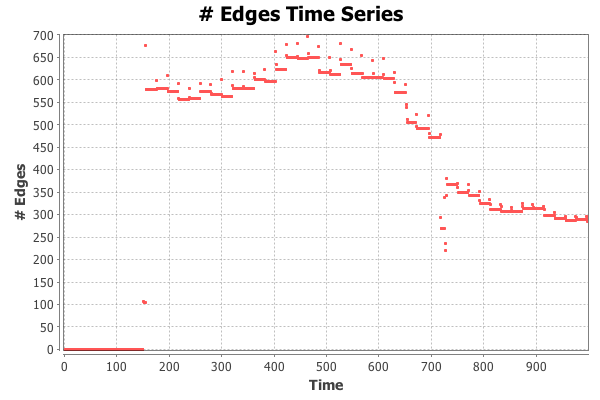
\includegraphics[scale=0.3]{plots/scribe_edges_face}
    \label{fig:scribe_edges_face}
    }
    \subfigure[Twitter] {
        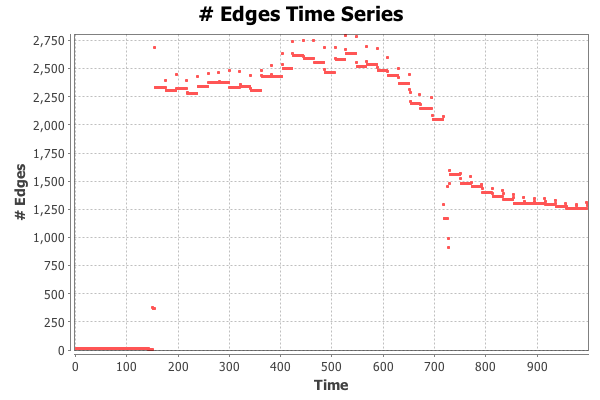
\includegraphics[scale=0.3]{plots/scribe_edges_twitter}
    \label{fig:scribe_edges_twitter}
    }
    \label{fig:scribe_edges}
    \caption{Plots describing the difference of number of edges in
        Scribe when using different subscription workloads.}
\end{figure}

Figure~\ref{fig:eval_directeddegree} shows directed degree in PolderCast
and Scribe. It confirms the much higher degree in PolderCast compared to
Scribe. It also a difference in average degree when using different
workloads. In particular, using the twitter workload seem to cause a
higher degree in both PolderCast and Scribe.  The difference is most
noticeable in Scribe, as the degree is quite low.  By using the
\emph{Statistics Component} in Gephi, we produce plots describing the
difference in number of edges in Scribe when using workloads from
Facebook and Twitter, seen in~\ref{fig:scribe_edges_face} and
Figure~\ref{fig:scribe_edges_twitter} respectively. It is clear that
using the workload from Twitter induces a much higher number of edges.
This might be indicative of a higher overlap in subscription interests,
increasing the number of tree structures being constructed. Such an
indication is also mentioned in~\cite{Setty:2012}. Furthermore, the
average degree are stable with regards to node churn, which might
indicate that the distribution of node degree does not diverge too much
from the mean. More specifically, there are few nodes with a very high
or a very low node degree. This decreases the likelihood of such a node
to leave the network due to churn, which would have a large impact on
the average value of node degree. The two plots seen in
Figure~\ref{fig:eval_directeddegree} also indicate that there is an even
balance between in-degree and out-degree of nodes, as they both have
similar values.

\begin{figure}[H]
    \thisfloatpagestyle{empty}
    \centering
        % GNUPLOT: LaTeX picture with Postscript
\begingroup
  \makeatletter
  \providecommand\color[2][]{%
    \GenericError{(gnuplot) \space\space\space\@spaces}{%
      Package color not loaded in conjunction with
      terminal option `colourtext'%
    }{See the gnuplot documentation for explanation.%
    }{Either use 'blacktext' in gnuplot or load the package
      color.sty in LaTeX.}%
    \renewcommand\color[2][]{}%
  }%
  \providecommand\includegraphics[2][]{%
    \GenericError{(gnuplot) \space\space\space\@spaces}{%
      Package graphicx or graphics not loaded%
    }{See the gnuplot documentation for explanation.%
    }{The gnuplot epslatex terminal needs graphicx.sty or graphics.sty.}%
    \renewcommand\includegraphics[2][]{}%
  }%
  \providecommand\rotatebox[2]{#2}%
  \@ifundefined{ifGPcolor}{%
    \newif\ifGPcolor
    \GPcolortrue
  }{}%
  \@ifundefined{ifGPblacktext}{%
    \newif\ifGPblacktext
    \GPblacktexttrue
  }{}%
  % define a \g@addto@macro without @ in the name:
  \let\gplgaddtomacro\g@addto@macro
  % define empty templates for all commands taking text:
  \gdef\gplbacktext{}%
  \gdef\gplfronttext{}%
  \makeatother
  \ifGPblacktext
    % no textcolor at all
    \def\colorrgb#1{}%
    \def\colorgray#1{}%
  \else
    % gray or color?
    \ifGPcolor
      \def\colorrgb#1{\color[rgb]{#1}}%
      \def\colorgray#1{\color[gray]{#1}}%
      \expandafter\def\csname LTw\endcsname{\color{white}}%
      \expandafter\def\csname LTb\endcsname{\color{black}}%
      \expandafter\def\csname LTa\endcsname{\color{black}}%
      \expandafter\def\csname LT0\endcsname{\color[rgb]{1,0,0}}%
      \expandafter\def\csname LT1\endcsname{\color[rgb]{0,1,0}}%
      \expandafter\def\csname LT2\endcsname{\color[rgb]{0,0,1}}%
      \expandafter\def\csname LT3\endcsname{\color[rgb]{1,0,1}}%
      \expandafter\def\csname LT4\endcsname{\color[rgb]{0,1,1}}%
      \expandafter\def\csname LT5\endcsname{\color[rgb]{1,1,0}}%
      \expandafter\def\csname LT6\endcsname{\color[rgb]{0,0,0}}%
      \expandafter\def\csname LT7\endcsname{\color[rgb]{1,0.3,0}}%
      \expandafter\def\csname LT8\endcsname{\color[rgb]{0.5,0.5,0.5}}%
    \else
      % gray
      \def\colorrgb#1{\color{black}}%
      \def\colorgray#1{\color[gray]{#1}}%
      \expandafter\def\csname LTw\endcsname{\color{white}}%
      \expandafter\def\csname LTb\endcsname{\color{black}}%
      \expandafter\def\csname LTa\endcsname{\color{black}}%
      \expandafter\def\csname LT0\endcsname{\color{black}}%
      \expandafter\def\csname LT1\endcsname{\color{black}}%
      \expandafter\def\csname LT2\endcsname{\color{black}}%
      \expandafter\def\csname LT3\endcsname{\color{black}}%
      \expandafter\def\csname LT4\endcsname{\color{black}}%
      \expandafter\def\csname LT5\endcsname{\color{black}}%
      \expandafter\def\csname LT6\endcsname{\color{black}}%
      \expandafter\def\csname LT7\endcsname{\color{black}}%
      \expandafter\def\csname LT8\endcsname{\color{black}}%
    \fi
  \fi
  \setlength{\unitlength}{0.0500bp}%
  \begin{picture}(7200.00,5040.00)%
    \gplgaddtomacro\gplbacktext{%
      \csname LTb\endcsname%
      \put(882,576){\makebox(0,0)[r]{\strut{} 0.1}}%
      \csname LTb\endcsname%
      \put(882,1638){\makebox(0,0)[r]{\strut{} 1}}%
      \csname LTb\endcsname%
      \put(882,2700){\makebox(0,0)[r]{\strut{} 10}}%
      \csname LTb\endcsname%
      \put(882,3761){\makebox(0,0)[r]{\strut{} 100}}%
      \csname LTb\endcsname%
      \put(882,4823){\makebox(0,0)[r]{\strut{} 1000}}%
      \csname LTb\endcsname%
      \put(990,396){\makebox(0,0){\strut{} 0}}%
      \csname LTb\endcsname%
      \put(1485,396){\makebox(0,0){\strut{} 100}}%
      \csname LTb\endcsname%
      \put(1980,396){\makebox(0,0){\strut{} 200}}%
      \csname LTb\endcsname%
      \put(2475,396){\makebox(0,0){\strut{} 300}}%
      \csname LTb\endcsname%
      \put(2970,396){\makebox(0,0){\strut{} 400}}%
      \csname LTb\endcsname%
      \put(3465,396){\makebox(0,0){\strut{} 500}}%
      \csname LTb\endcsname%
      \put(3959,396){\makebox(0,0){\strut{} 600}}%
      \csname LTb\endcsname%
      \put(4454,396){\makebox(0,0){\strut{} 700}}%
      \csname LTb\endcsname%
      \put(4949,396){\makebox(0,0){\strut{} 800}}%
      \csname LTb\endcsname%
      \put(5444,396){\makebox(0,0){\strut{} 900}}%
      \csname LTb\endcsname%
      \put(5939,396){\makebox(0,0){\strut{} 1000}}%
      \put(6047,576){\makebox(0,0)[l]{\strut{} 0}}%
      \put(6047,1001){\makebox(0,0)[l]{\strut{} 100}}%
      \put(6047,1425){\makebox(0,0)[l]{\strut{} 200}}%
      \put(6047,1850){\makebox(0,0)[l]{\strut{} 300}}%
      \put(6047,2275){\makebox(0,0)[l]{\strut{} 400}}%
      \put(6047,2700){\makebox(0,0)[l]{\strut{} 500}}%
      \put(6047,3124){\makebox(0,0)[l]{\strut{} 600}}%
      \put(6047,3549){\makebox(0,0)[l]{\strut{} 700}}%
      \put(6047,3974){\makebox(0,0)[l]{\strut{} 800}}%
      \put(6047,4398){\makebox(0,0)[l]{\strut{} 900}}%
      \put(6047,4823){\makebox(0,0)[l]{\strut{} 1000}}%
      \put(144,2699){\rotatebox{-270}{\makebox(0,0){\strut{}In-degree}}}%
      \put(6784,2699){\rotatebox{-270}{\makebox(0,0){\strut{}Network Size}}}%
      \put(3464,126){\makebox(0,0){\strut{}Reporter Intervals}}%
    }%
    \gplgaddtomacro\gplfronttext{%
      \csname LTb\endcsname%
      \put(5120,1449){\makebox(0,0)[r]{\strut{}PolderCast (Facebook)}}%
      \csname LTb\endcsname%
      \put(5120,1269){\makebox(0,0)[r]{\strut{}PolderCast (Twitter)}}%
      \csname LTb\endcsname%
      \put(5120,1089){\makebox(0,0)[r]{\strut{}Scribe (Facebook)}}%
      \csname LTb\endcsname%
      \put(5120,909){\makebox(0,0)[r]{\strut{}Scribe (Twitter)}}%
      \csname LTb\endcsname%
      \put(5120,729){\makebox(0,0)[r]{\strut{}Network Size}}%
    }%
    \gplbacktext
    \put(0,0){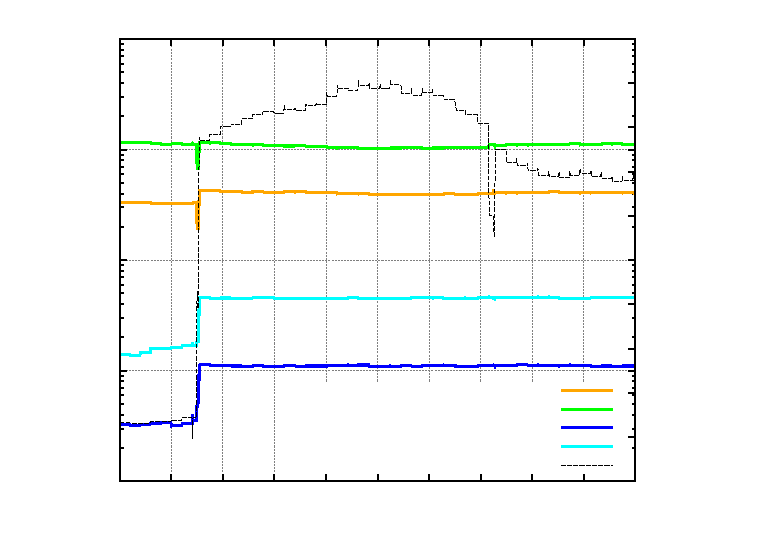
\includegraphics{eval_indegree}}%
    \gplfronttext
  \end{picture}%
\endgroup

        \label{fig:eval_indegree}
        % GNUPLOT: LaTeX picture with Postscript
\begingroup
  \makeatletter
  \providecommand\color[2][]{%
    \GenericError{(gnuplot) \space\space\space\@spaces}{%
      Package color not loaded in conjunction with
      terminal option `colourtext'%
    }{See the gnuplot documentation for explanation.%
    }{Either use 'blacktext' in gnuplot or load the package
      color.sty in LaTeX.}%
    \renewcommand\color[2][]{}%
  }%
  \providecommand\includegraphics[2][]{%
    \GenericError{(gnuplot) \space\space\space\@spaces}{%
      Package graphicx or graphics not loaded%
    }{See the gnuplot documentation for explanation.%
    }{The gnuplot epslatex terminal needs graphicx.sty or graphics.sty.}%
    \renewcommand\includegraphics[2][]{}%
  }%
  \providecommand\rotatebox[2]{#2}%
  \@ifundefined{ifGPcolor}{%
    \newif\ifGPcolor
    \GPcolortrue
  }{}%
  \@ifundefined{ifGPblacktext}{%
    \newif\ifGPblacktext
    \GPblacktexttrue
  }{}%
  % define a \g@addto@macro without @ in the name:
  \let\gplgaddtomacro\g@addto@macro
  % define empty templates for all commands taking text:
  \gdef\gplbacktext{}%
  \gdef\gplfronttext{}%
  \makeatother
  \ifGPblacktext
    % no textcolor at all
    \def\colorrgb#1{}%
    \def\colorgray#1{}%
  \else
    % gray or color?
    \ifGPcolor
      \def\colorrgb#1{\color[rgb]{#1}}%
      \def\colorgray#1{\color[gray]{#1}}%
      \expandafter\def\csname LTw\endcsname{\color{white}}%
      \expandafter\def\csname LTb\endcsname{\color{black}}%
      \expandafter\def\csname LTa\endcsname{\color{black}}%
      \expandafter\def\csname LT0\endcsname{\color[rgb]{1,0,0}}%
      \expandafter\def\csname LT1\endcsname{\color[rgb]{0,1,0}}%
      \expandafter\def\csname LT2\endcsname{\color[rgb]{0,0,1}}%
      \expandafter\def\csname LT3\endcsname{\color[rgb]{1,0,1}}%
      \expandafter\def\csname LT4\endcsname{\color[rgb]{0,1,1}}%
      \expandafter\def\csname LT5\endcsname{\color[rgb]{1,1,0}}%
      \expandafter\def\csname LT6\endcsname{\color[rgb]{0,0,0}}%
      \expandafter\def\csname LT7\endcsname{\color[rgb]{1,0.3,0}}%
      \expandafter\def\csname LT8\endcsname{\color[rgb]{0.5,0.5,0.5}}%
    \else
      % gray
      \def\colorrgb#1{\color{black}}%
      \def\colorgray#1{\color[gray]{#1}}%
      \expandafter\def\csname LTw\endcsname{\color{white}}%
      \expandafter\def\csname LTb\endcsname{\color{black}}%
      \expandafter\def\csname LTa\endcsname{\color{black}}%
      \expandafter\def\csname LT0\endcsname{\color{black}}%
      \expandafter\def\csname LT1\endcsname{\color{black}}%
      \expandafter\def\csname LT2\endcsname{\color{black}}%
      \expandafter\def\csname LT3\endcsname{\color{black}}%
      \expandafter\def\csname LT4\endcsname{\color{black}}%
      \expandafter\def\csname LT5\endcsname{\color{black}}%
      \expandafter\def\csname LT6\endcsname{\color{black}}%
      \expandafter\def\csname LT7\endcsname{\color{black}}%
      \expandafter\def\csname LT8\endcsname{\color{black}}%
    \fi
  \fi
  \setlength{\unitlength}{0.0500bp}%
  \begin{picture}(7200.00,5040.00)%
    \gplgaddtomacro\gplbacktext{%
      \csname LTb\endcsname%
      \put(882,576){\makebox(0,0)[r]{\strut{} 0.1}}%
      \csname LTb\endcsname%
      \put(882,1638){\makebox(0,0)[r]{\strut{} 1}}%
      \csname LTb\endcsname%
      \put(882,2700){\makebox(0,0)[r]{\strut{} 10}}%
      \csname LTb\endcsname%
      \put(882,3761){\makebox(0,0)[r]{\strut{} 100}}%
      \csname LTb\endcsname%
      \put(882,4823){\makebox(0,0)[r]{\strut{} 1000}}%
      \csname LTb\endcsname%
      \put(990,396){\makebox(0,0){\strut{} 0}}%
      \csname LTb\endcsname%
      \put(1485,396){\makebox(0,0){\strut{} 100}}%
      \csname LTb\endcsname%
      \put(1980,396){\makebox(0,0){\strut{} 200}}%
      \csname LTb\endcsname%
      \put(2475,396){\makebox(0,0){\strut{} 300}}%
      \csname LTb\endcsname%
      \put(2970,396){\makebox(0,0){\strut{} 400}}%
      \csname LTb\endcsname%
      \put(3465,396){\makebox(0,0){\strut{} 500}}%
      \csname LTb\endcsname%
      \put(3959,396){\makebox(0,0){\strut{} 600}}%
      \csname LTb\endcsname%
      \put(4454,396){\makebox(0,0){\strut{} 700}}%
      \csname LTb\endcsname%
      \put(4949,396){\makebox(0,0){\strut{} 800}}%
      \csname LTb\endcsname%
      \put(5444,396){\makebox(0,0){\strut{} 900}}%
      \csname LTb\endcsname%
      \put(5939,396){\makebox(0,0){\strut{} 1000}}%
      \put(6047,576){\makebox(0,0)[l]{\strut{} 0}}%
      \put(6047,1001){\makebox(0,0)[l]{\strut{} 100}}%
      \put(6047,1425){\makebox(0,0)[l]{\strut{} 200}}%
      \put(6047,1850){\makebox(0,0)[l]{\strut{} 300}}%
      \put(6047,2275){\makebox(0,0)[l]{\strut{} 400}}%
      \put(6047,2700){\makebox(0,0)[l]{\strut{} 500}}%
      \put(6047,3124){\makebox(0,0)[l]{\strut{} 600}}%
      \put(6047,3549){\makebox(0,0)[l]{\strut{} 700}}%
      \put(6047,3974){\makebox(0,0)[l]{\strut{} 800}}%
      \put(6047,4398){\makebox(0,0)[l]{\strut{} 900}}%
      \put(6047,4823){\makebox(0,0)[l]{\strut{} 1000}}%
      \put(144,2699){\rotatebox{-270}{\makebox(0,0){\strut{}Avg. Out-Degree}}}%
      \put(6784,2699){\rotatebox{-270}{\makebox(0,0){\strut{}Network Size}}}%
      \put(3464,126){\makebox(0,0){\strut{}Reporter Intervals}}%
    }%
    \gplgaddtomacro\gplfronttext{%
      \csname LTb\endcsname%
      \put(5120,1449){\makebox(0,0)[r]{\strut{}PolderCast (Facebook)}}%
      \csname LTb\endcsname%
      \put(5120,1269){\makebox(0,0)[r]{\strut{}PolderCast (Twitter)}}%
      \csname LTb\endcsname%
      \put(5120,1089){\makebox(0,0)[r]{\strut{}Scribe (Facebook)}}%
      \csname LTb\endcsname%
      \put(5120,909){\makebox(0,0)[r]{\strut{}Scribe (Twitter)}}%
      \csname LTb\endcsname%
      \put(5120,729){\makebox(0,0)[r]{\strut{}Network Size}}%
    }%
    \gplbacktext
    \put(0,0){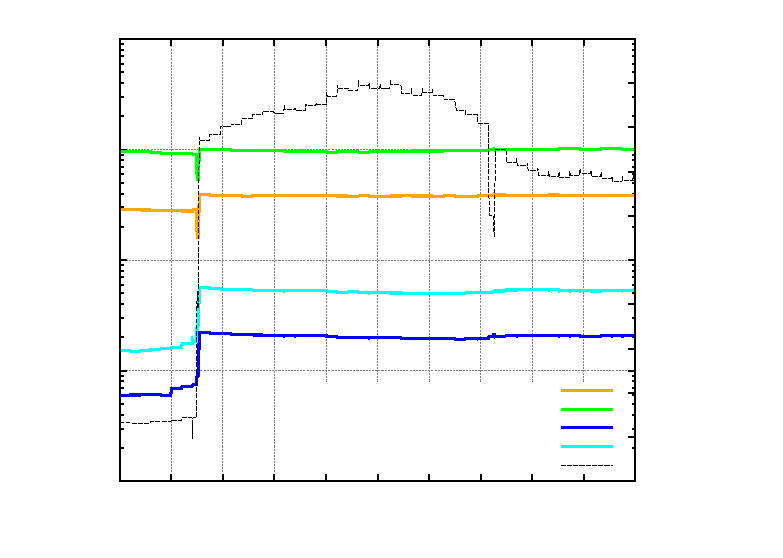
\includegraphics{eval_outdegree}}%
    \gplfronttext
  \end{picture}%
\endgroup

        \label{fig:eval_outdegree}
    \caption{Avg. Directed Degrees of PolderCast and Scribe}
    \label{fig:eval_directeddegree}
\end{figure}


% \subsection{Clustering Coefficient}

Average Clustering coefficient is described in Figure~\ref{fig:eval_cc}.
The average is calculated by dividing the \emph{local clustering
    coefficient} of each node, and divide it by the number of nodes in
the overlay. As expected, PolderCast has a higher clustering
coefficient. However, it is worth noting that the clustering coefficient
of PolderCast seems relatively unaffected by using different workloads,
while in Scribe the clustering coefficient goes up when using the
Twitter dataset for subscriptions. Again, this is a natural consequence
of the much higher number of edges in Scribe when running the Twitter
workload. The fact that PolderCast has a higher clustering coefficient
is hardly surprising, as the we know from Chapter~\ref{ch:vizpub} that
the overlay in PolderCast is more dense.

\begin{figure}[H]
    \centering
    \thisfloatpagestyle{empty}
    % GNUPLOT: LaTeX picture with Postscript
\begingroup
  \makeatletter
  \providecommand\color[2][]{%
    \GenericError{(gnuplot) \space\space\space\@spaces}{%
      Package color not loaded in conjunction with
      terminal option `colourtext'%
    }{See the gnuplot documentation for explanation.%
    }{Either use 'blacktext' in gnuplot or load the package
      color.sty in LaTeX.}%
    \renewcommand\color[2][]{}%
  }%
  \providecommand\includegraphics[2][]{%
    \GenericError{(gnuplot) \space\space\space\@spaces}{%
      Package graphicx or graphics not loaded%
    }{See the gnuplot documentation for explanation.%
    }{The gnuplot epslatex terminal needs graphicx.sty or graphics.sty.}%
    \renewcommand\includegraphics[2][]{}%
  }%
  \providecommand\rotatebox[2]{#2}%
  \@ifundefined{ifGPcolor}{%
    \newif\ifGPcolor
    \GPcolortrue
  }{}%
  \@ifundefined{ifGPblacktext}{%
    \newif\ifGPblacktext
    \GPblacktexttrue
  }{}%
  % define a \g@addto@macro without @ in the name:
  \let\gplgaddtomacro\g@addto@macro
  % define empty templates for all commands taking text:
  \gdef\gplbacktext{}%
  \gdef\gplfronttext{}%
  \makeatother
  \ifGPblacktext
    % no textcolor at all
    \def\colorrgb#1{}%
    \def\colorgray#1{}%
  \else
    % gray or color?
    \ifGPcolor
      \def\colorrgb#1{\color[rgb]{#1}}%
      \def\colorgray#1{\color[gray]{#1}}%
      \expandafter\def\csname LTw\endcsname{\color{white}}%
      \expandafter\def\csname LTb\endcsname{\color{black}}%
      \expandafter\def\csname LTa\endcsname{\color{black}}%
      \expandafter\def\csname LT0\endcsname{\color[rgb]{1,0,0}}%
      \expandafter\def\csname LT1\endcsname{\color[rgb]{0,1,0}}%
      \expandafter\def\csname LT2\endcsname{\color[rgb]{0,0,1}}%
      \expandafter\def\csname LT3\endcsname{\color[rgb]{1,0,1}}%
      \expandafter\def\csname LT4\endcsname{\color[rgb]{0,1,1}}%
      \expandafter\def\csname LT5\endcsname{\color[rgb]{1,1,0}}%
      \expandafter\def\csname LT6\endcsname{\color[rgb]{0,0,0}}%
      \expandafter\def\csname LT7\endcsname{\color[rgb]{1,0.3,0}}%
      \expandafter\def\csname LT8\endcsname{\color[rgb]{0.5,0.5,0.5}}%
    \else
      % gray
      \def\colorrgb#1{\color{black}}%
      \def\colorgray#1{\color[gray]{#1}}%
      \expandafter\def\csname LTw\endcsname{\color{white}}%
      \expandafter\def\csname LTb\endcsname{\color{black}}%
      \expandafter\def\csname LTa\endcsname{\color{black}}%
      \expandafter\def\csname LT0\endcsname{\color{black}}%
      \expandafter\def\csname LT1\endcsname{\color{black}}%
      \expandafter\def\csname LT2\endcsname{\color{black}}%
      \expandafter\def\csname LT3\endcsname{\color{black}}%
      \expandafter\def\csname LT4\endcsname{\color{black}}%
      \expandafter\def\csname LT5\endcsname{\color{black}}%
      \expandafter\def\csname LT6\endcsname{\color{black}}%
      \expandafter\def\csname LT7\endcsname{\color{black}}%
      \expandafter\def\csname LT8\endcsname{\color{black}}%
    \fi
  \fi
  \setlength{\unitlength}{0.0500bp}%
  \begin{picture}(7200.00,5040.00)%
    \gplgaddtomacro\gplbacktext{%
      \csname LTb\endcsname%
      \put(1342,704){\makebox(0,0)[r]{\strut{} 0.0001}}%
      \csname LTb\endcsname%
      \put(1342,1722){\makebox(0,0)[r]{\strut{} 0.001}}%
      \csname LTb\endcsname%
      \put(1342,2740){\makebox(0,0)[r]{\strut{} 0.01}}%
      \csname LTb\endcsname%
      \put(1342,3757){\makebox(0,0)[r]{\strut{} 0.1}}%
      \csname LTb\endcsname%
      \put(1342,4775){\makebox(0,0)[r]{\strut{} 1}}%
      \csname LTb\endcsname%
      \put(1474,484){\makebox(0,0){\strut{} 0}}%
      \csname LTb\endcsname%
      \put(1893,484){\makebox(0,0){\strut{} 100}}%
      \csname LTb\endcsname%
      \put(2311,484){\makebox(0,0){\strut{} 200}}%
      \csname LTb\endcsname%
      \put(2730,484){\makebox(0,0){\strut{} 300}}%
      \csname LTb\endcsname%
      \put(3148,484){\makebox(0,0){\strut{} 400}}%
      \csname LTb\endcsname%
      \put(3567,484){\makebox(0,0){\strut{} 500}}%
      \csname LTb\endcsname%
      \put(3985,484){\makebox(0,0){\strut{} 600}}%
      \csname LTb\endcsname%
      \put(4404,484){\makebox(0,0){\strut{} 700}}%
      \csname LTb\endcsname%
      \put(4822,484){\makebox(0,0){\strut{} 800}}%
      \csname LTb\endcsname%
      \put(5241,484){\makebox(0,0){\strut{} 900}}%
      \csname LTb\endcsname%
      \put(5659,484){\makebox(0,0){\strut{} 1000}}%
      \put(5791,704){\makebox(0,0)[l]{\strut{} 0}}%
      \put(5791,1111){\makebox(0,0)[l]{\strut{} 100}}%
      \put(5791,1518){\makebox(0,0)[l]{\strut{} 200}}%
      \put(5791,1925){\makebox(0,0)[l]{\strut{} 300}}%
      \put(5791,2332){\makebox(0,0)[l]{\strut{} 400}}%
      \put(5791,2740){\makebox(0,0)[l]{\strut{} 500}}%
      \put(5791,3147){\makebox(0,0)[l]{\strut{} 600}}%
      \put(5791,3554){\makebox(0,0)[l]{\strut{} 700}}%
      \put(5791,3961){\makebox(0,0)[l]{\strut{} 800}}%
      \put(5791,4368){\makebox(0,0)[l]{\strut{} 900}}%
      \put(5791,4775){\makebox(0,0)[l]{\strut{} 1000}}%
      \put(176,2739){\rotatebox{-270}{\makebox(0,0){\strut{}Avg. Clustering Coefficient}}}%
      \put(6692,2739){\rotatebox{-270}{\makebox(0,0){\strut{}Network Size}}}%
      \put(3566,154){\makebox(0,0){\strut{}Reporter Intervals}}%
    }%
    \gplgaddtomacro\gplfronttext{%
      \csname LTb\endcsname%
      \put(4672,1757){\makebox(0,0)[r]{\strut{}PolderCast (Facebook)}}%
      \csname LTb\endcsname%
      \put(4672,1537){\makebox(0,0)[r]{\strut{}PolderCast (Twitter)}}%
      \csname LTb\endcsname%
      \put(4672,1317){\makebox(0,0)[r]{\strut{}Scribe (Facebook)}}%
      \csname LTb\endcsname%
      \put(4672,1097){\makebox(0,0)[r]{\strut{}Scribe (Twitter)}}%
      \csname LTb\endcsname%
      \put(4672,877){\makebox(0,0)[r]{\strut{}Network Size}}%
    }%
    \gplbacktext
    \put(0,0){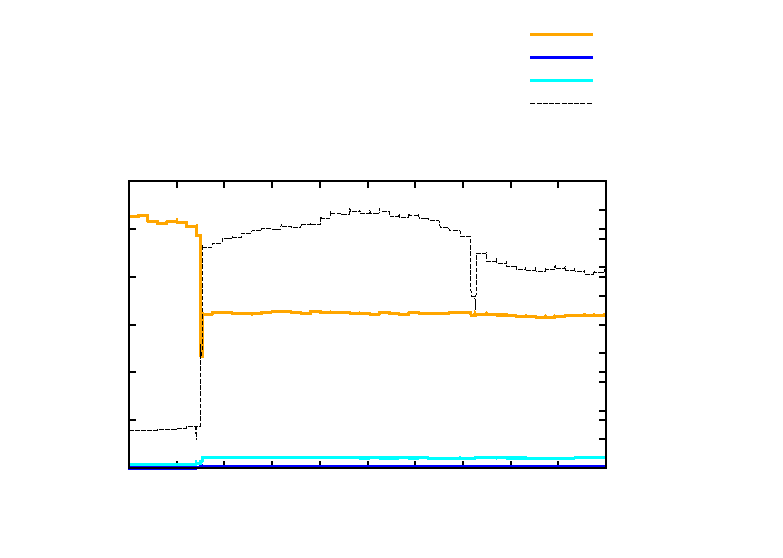
\includegraphics{eval_cc}}%
    \gplfronttext
  \end{picture}%
\endgroup

    \caption{Avg. Clustering Coefficient of PolderCast and Scribe}
    \label{fig:eval_cc}
\end{figure}

%\subsection{Centralities}

Results of calculating centrality metrics can be seen in
Figure~\ref{fig:eval_betweenness}, Figure~\ref{fig:eval_closeness} and
Figure~\ref{fig:eval_eccentricity}. Again it can be observed in all
plots, that the values of the metric calculations in Scribe diverge
depending on the what workload is being used for subscriptions. No such
discrepancy can be seen in PolderCast.

Figure~\ref{fig:eval_betweenness} describes the average betweenness
centrality of nodes. Although PolderCast have a high betweenness, the
values do not seem to fluctuate too much depending on the workload. In
Scribe however, we see the mentioned discrepancy. Using the workload
from Twitter causes much higher values. Indeed, nodes in the Scribe
overlay have the highest average betweenness centralities when running
this workload. This could be an indication that Scribe does not scale
well in terms of betweenness as the number of edges increases. This
could impact the performance of the pub/sub system when running certain
workloads.

The average closeness centrality of nodes can be seen in
Figure~\ref{fig:eval_closeness}. Here Scribe populate the top values as
using both workloads, although the discrepancy of results depending on
the data set used is still higher than in PolderCast. This is hardly
surprising, as closeness is a measure between the distance of a node
$n$ and any other nodes in the system. Seeing that the overlay in
PolderCast is much more dense as well as having a shorter diameter, we
expect nodes in PolderCast to have a lower closeness centrality as
well.

Figure~\ref{fig:eval_eccentricity} describes the average eccentricity
centrality of nodes. The result of running the eccentricity metric seems
to be comparable with the results in Figure~\ref{fig:eval_closeness}.
Again, running Scribe has the highest eccentricity when running the
Twitter workload. When running the Facebook workload however, Scribe
actually has a lower average eccentricity than compared to PolderCast.

The low number of edges and relative high number of
disconnected nodes seen in Scribe when running the workload from
Facebook might effect the results. It would be interesting to see what
is the cause of this. One possible reason might be the scale of the
experiment, as we could only run 2000 nodes for this thesis. With more
time to spare, we would run further experiments at different scales in
order to test the effects. However, much work is needed before this is
possible, as \demo{} is still a young tool. We describe such future work
in Chapter~\ref{ch:conclusion} where we also address some of the
limitations of \demo{}

The low number of edges in Scribe, might also be caused by the amount of
churn in the system, as the dissemination structure in Scribe are , in
theory, brittle. Indeed, by running an experiment without churn, we were
able to visually confirm that the overlay in scribe was composed of only
one connected component by quickly inspecting the graph in Gephi. This
confirm in practice the brittleness of the overlay structures of Scribe,
but this needs further investigation. This investigation should include
adjusting the churn rate in order to see the effects of the overlays,
and perhaps compare the density of the graph, looking at the number of
edges formed as well as evaluating its connectivity.

\section{Summary}

It should be repeated that \demo{} is indeed a prototype, and there
might still be software bugs which affect the results. But the intention
of this chapter lies not only in producing results, but also test
\demo{} as a platform for evaluation of pub/sub systems. Although there
are many issues which still needs to be addressed, we believe the
potential for such a tool should be explored.

Our main concern when developing \demo{} was being able to visualize
pub/sub systems, but with this chapter we believe we provide some
examples to back up the claim that \demo{} can be used as a tool for
evaluation as well as visualization. We believe such a tool would be of
great benefit to the research community, and we hope the extendability
of Gephi through its ecosystem of plugins can encourage researcher to share
more code between them.

% Currently, the collector does not provide us any information regarding
% the \emph{variance} or \emph{standard deviation} of the data being
% collected. However, using Gephi we can produce plots describing the
% distribution of values for a particular interval. As averages remain
% stable after the initial network spike, this should tell us something
% about how precise these averages are. In Figure~\ref{fig:betw_distr}
% we see such plots for the betweenness centralities in PolderCast and
% Scribe at interval 1000, running both the Facebook and Twitter
% datasets.

\begin{figure}[H]
    \centering
    \thisfloatpagestyle{empty}
    % GNUPLOT: LaTeX picture with Postscript
\begingroup
  \makeatletter
  \providecommand\color[2][]{%
    \GenericError{(gnuplot) \space\space\space\@spaces}{%
      Package color not loaded in conjunction with
      terminal option `colourtext'%
    }{See the gnuplot documentation for explanation.%
    }{Either use 'blacktext' in gnuplot or load the package
      color.sty in LaTeX.}%
    \renewcommand\color[2][]{}%
  }%
  \providecommand\includegraphics[2][]{%
    \GenericError{(gnuplot) \space\space\space\@spaces}{%
      Package graphicx or graphics not loaded%
    }{See the gnuplot documentation for explanation.%
    }{The gnuplot epslatex terminal needs graphicx.sty or graphics.sty.}%
    \renewcommand\includegraphics[2][]{}%
  }%
  \providecommand\rotatebox[2]{#2}%
  \@ifundefined{ifGPcolor}{%
    \newif\ifGPcolor
    \GPcolortrue
  }{}%
  \@ifundefined{ifGPblacktext}{%
    \newif\ifGPblacktext
    \GPblacktexttrue
  }{}%
  % define a \g@addto@macro without @ in the name:
  \let\gplgaddtomacro\g@addto@macro
  % define empty templates for all commands taking text:
  \gdef\gplbacktext{}%
  \gdef\gplfronttext{}%
  \makeatother
  \ifGPblacktext
    % no textcolor at all
    \def\colorrgb#1{}%
    \def\colorgray#1{}%
  \else
    % gray or color?
    \ifGPcolor
      \def\colorrgb#1{\color[rgb]{#1}}%
      \def\colorgray#1{\color[gray]{#1}}%
      \expandafter\def\csname LTw\endcsname{\color{white}}%
      \expandafter\def\csname LTb\endcsname{\color{black}}%
      \expandafter\def\csname LTa\endcsname{\color{black}}%
      \expandafter\def\csname LT0\endcsname{\color[rgb]{1,0,0}}%
      \expandafter\def\csname LT1\endcsname{\color[rgb]{0,1,0}}%
      \expandafter\def\csname LT2\endcsname{\color[rgb]{0,0,1}}%
      \expandafter\def\csname LT3\endcsname{\color[rgb]{1,0,1}}%
      \expandafter\def\csname LT4\endcsname{\color[rgb]{0,1,1}}%
      \expandafter\def\csname LT5\endcsname{\color[rgb]{1,1,0}}%
      \expandafter\def\csname LT6\endcsname{\color[rgb]{0,0,0}}%
      \expandafter\def\csname LT7\endcsname{\color[rgb]{1,0.3,0}}%
      \expandafter\def\csname LT8\endcsname{\color[rgb]{0.5,0.5,0.5}}%
    \else
      % gray
      \def\colorrgb#1{\color{black}}%
      \def\colorgray#1{\color[gray]{#1}}%
      \expandafter\def\csname LTw\endcsname{\color{white}}%
      \expandafter\def\csname LTb\endcsname{\color{black}}%
      \expandafter\def\csname LTa\endcsname{\color{black}}%
      \expandafter\def\csname LT0\endcsname{\color{black}}%
      \expandafter\def\csname LT1\endcsname{\color{black}}%
      \expandafter\def\csname LT2\endcsname{\color{black}}%
      \expandafter\def\csname LT3\endcsname{\color{black}}%
      \expandafter\def\csname LT4\endcsname{\color{black}}%
      \expandafter\def\csname LT5\endcsname{\color{black}}%
      \expandafter\def\csname LT6\endcsname{\color{black}}%
      \expandafter\def\csname LT7\endcsname{\color{black}}%
      \expandafter\def\csname LT8\endcsname{\color{black}}%
    \fi
  \fi
  \setlength{\unitlength}{0.0500bp}%
  \begin{picture}(7200.00,5040.00)%
    \gplgaddtomacro\gplbacktext{%
      \csname LTb\endcsname%
      \put(1078,704){\makebox(0,0)[r]{\strut{} 0}}%
      \put(1078,1163){\makebox(0,0)[r]{\strut{} 1000}}%
      \put(1078,1621){\makebox(0,0)[r]{\strut{} 2000}}%
      \put(1078,2080){\makebox(0,0)[r]{\strut{} 3000}}%
      \put(1078,2538){\makebox(0,0)[r]{\strut{} 4000}}%
      \put(1078,2997){\makebox(0,0)[r]{\strut{} 5000}}%
      \put(1078,3455){\makebox(0,0)[r]{\strut{} 6000}}%
      \put(1210,484){\makebox(0,0){\strut{} 0}}%
      \put(1655,484){\makebox(0,0){\strut{} 100}}%
      \put(2100,484){\makebox(0,0){\strut{} 200}}%
      \put(2545,484){\makebox(0,0){\strut{} 300}}%
      \put(2990,484){\makebox(0,0){\strut{} 400}}%
      \put(3435,484){\makebox(0,0){\strut{} 500}}%
      \put(3879,484){\makebox(0,0){\strut{} 600}}%
      \put(4324,484){\makebox(0,0){\strut{} 700}}%
      \put(4769,484){\makebox(0,0){\strut{} 800}}%
      \put(5214,484){\makebox(0,0){\strut{} 900}}%
      \put(5659,484){\makebox(0,0){\strut{} 1000}}%
      \put(5791,704){\makebox(0,0)[l]{\strut{} 0}}%
      \put(5791,979){\makebox(0,0)[l]{\strut{} 100}}%
      \put(5791,1254){\makebox(0,0)[l]{\strut{} 200}}%
      \put(5791,1529){\makebox(0,0)[l]{\strut{} 300}}%
      \put(5791,1804){\makebox(0,0)[l]{\strut{} 400}}%
      \put(5791,2080){\makebox(0,0)[l]{\strut{} 500}}%
      \put(5791,2355){\makebox(0,0)[l]{\strut{} 600}}%
      \put(5791,2630){\makebox(0,0)[l]{\strut{} 700}}%
      \put(5791,2905){\makebox(0,0)[l]{\strut{} 800}}%
      \put(5791,3180){\makebox(0,0)[l]{\strut{} 900}}%
      \put(5791,3455){\makebox(0,0)[l]{\strut{} 1000}}%
      \put(176,2079){\rotatebox{-270}{\makebox(0,0){\strut{}Betweenness Centrality}}}%
      \put(6692,2079){\rotatebox{-270}{\makebox(0,0){\strut{}Network Size}}}%
      \put(3434,154){\makebox(0,0){\strut{}Reporter Intervals}}%
    }%
    \gplgaddtomacro\gplfronttext{%
      \csname LTb\endcsname%
      \put(4804,4867){\makebox(0,0)[r]{\strut{}PolderCast (Facebook)}}%
      \csname LTb\endcsname%
      \put(4804,4647){\makebox(0,0)[r]{\strut{}PolderCast (Twitter)}}%
      \csname LTb\endcsname%
      \put(4804,4427){\makebox(0,0)[r]{\strut{}Scribe (Facebook)}}%
      \csname LTb\endcsname%
      \put(4804,4207){\makebox(0,0)[r]{\strut{}Scribe (Twitter)}}%
      \csname LTb\endcsname%
      \put(4804,3987){\makebox(0,0)[r]{\strut{}Network Size}}%
    }%
    \gplbacktext
    \put(0,0){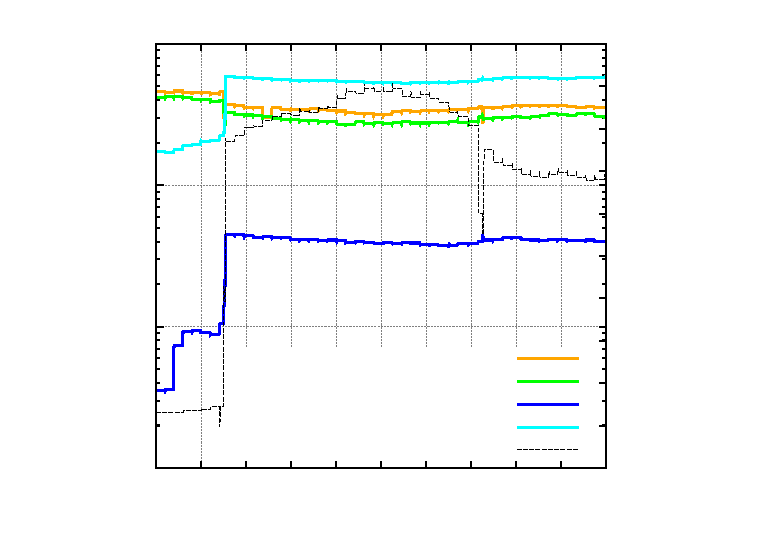
\includegraphics{eval_betweenness}}%
    \gplfronttext
  \end{picture}%
\endgroup

    \caption{Avg. Betweenness Centrality of PolderCast and Scribe}
    \label{fig:eval_betweenness}
\end{figure}

% \begin{figure}[H]
% \vspace{-60pt}
%     \centering
%     \thisfloatpagestyle{empty}
%     \subfigure[PolderCast (Twitter)]{
%     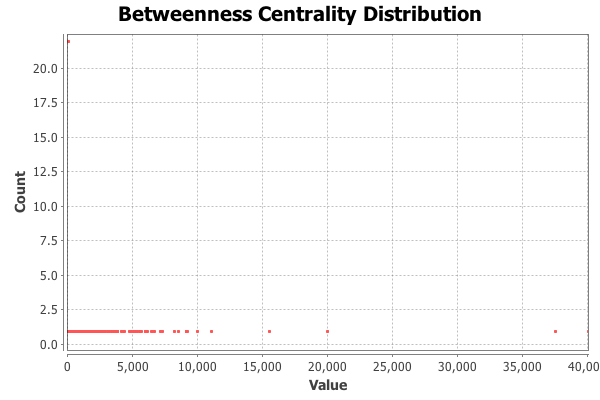
\includegraphics[scale=0.3]{plots/polder_betw_distr_tw}
% }
%     \subfigure[Scribe (Twitter)]{
%     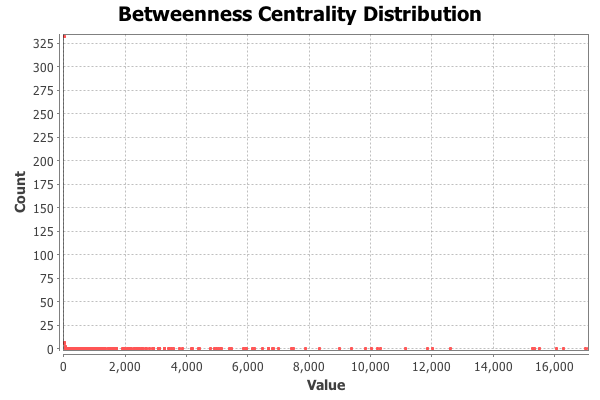
\includegraphics[scale=0.3]{plots/scribe_betw_distr_tw}
% }
%     \subfigure[PolderCast (Facebook)]{
%     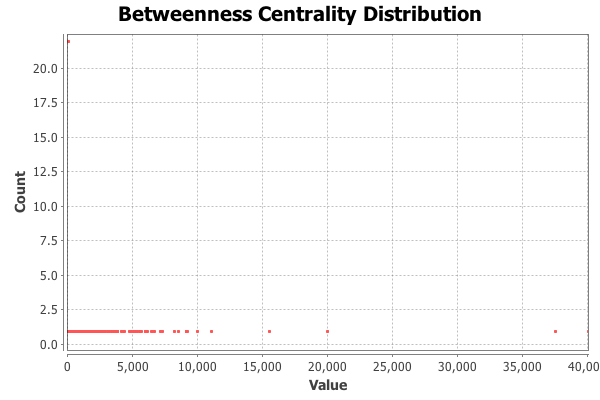
\includegraphics[scale=0.3]{plots/polder_betw_distr_face}
% }
%     \subfigure[Scribe (Facebook)]{
%     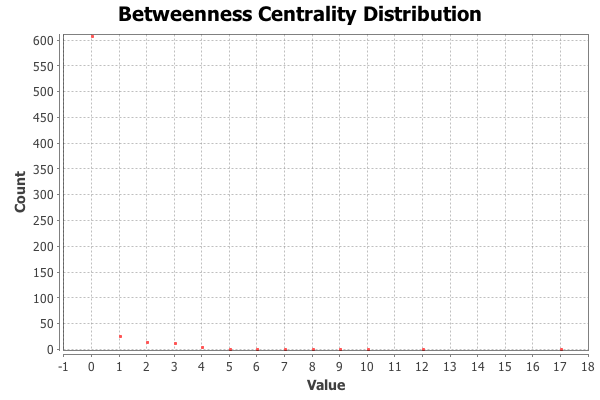
\includegraphics[scale=0.3]{plots/scribe_betw_distr_face}
% }
%     \label{fig:betw_distr}
%     \caption{Plots showing distribution of betweenness in PolderCast and
%     Scribe at reporter interval 1000}
% \end{figure}

% \begin{figure}[H]
%     \centering
%     \thisfloatpagestyle{empty}
%     \subfigure[PolderCast (Twitter)]{
%     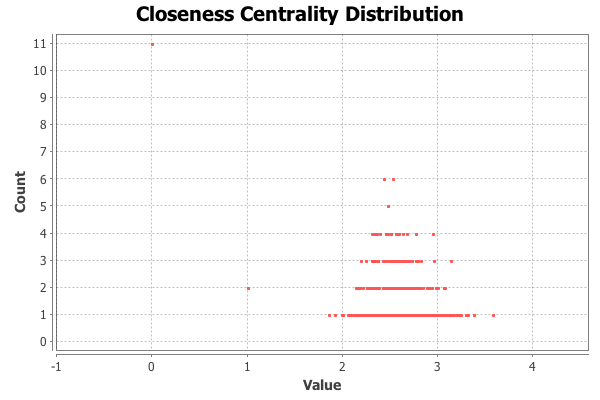
\includegraphics[scale=0.3]{plots/polder_clos_distr_tw}
% }
%     \subfigure[Scribe (Twitter)]{
%     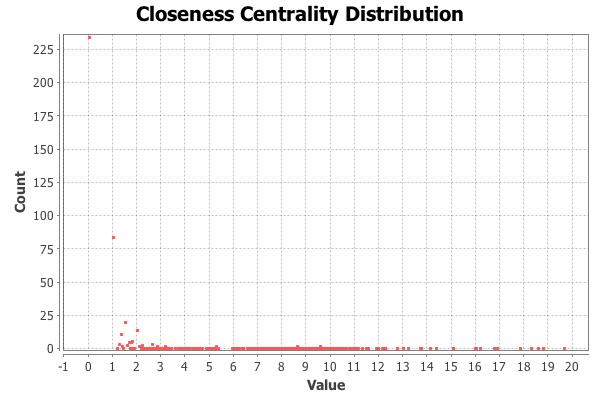
\includegraphics[scale=0.3]{plots/scribe_clos_distr_tw}
% }
%     \subfigure[PolderCast (Facebook)]{
%     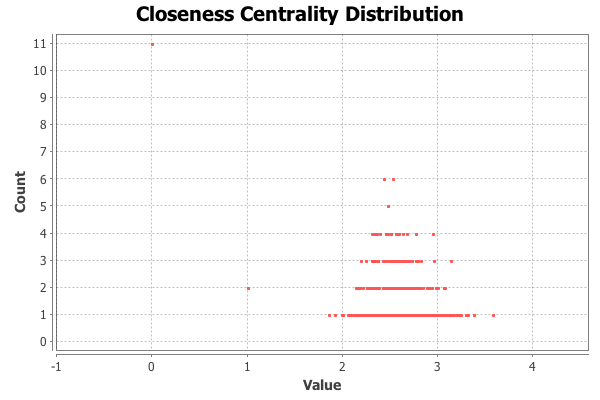
\includegraphics[scale=0.3]{plots/polder_clos_distr_face}
% }
%     \subfigure[Scribe (Facebook)]{
%     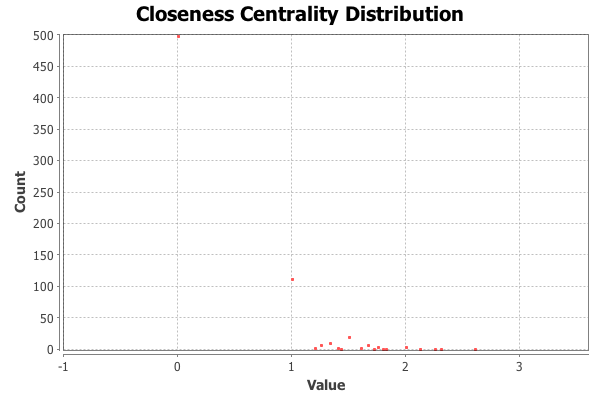
\includegraphics[scale=0.3]{plots/scribe_clos_distr_face}
% }
%     \label{fig:betw_distr}
%     \caption{Plots showing distribution of closeness in PolderCast and
%     Scribe at reporter interval 1000}
% \end{figure}

% \begin{figure}[H]
%     \centering
%     \thisfloatpagestyle{empty}
%     \subfigure[PolderCast (Twitter)]{
%     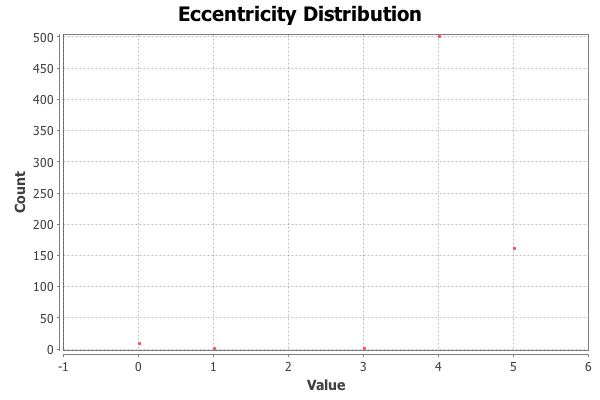
\includegraphics[scale=0.3]{plots/polder_ecc_distr_tw}
% }
%     \subfigure[Scribe (Twitter)]{
%     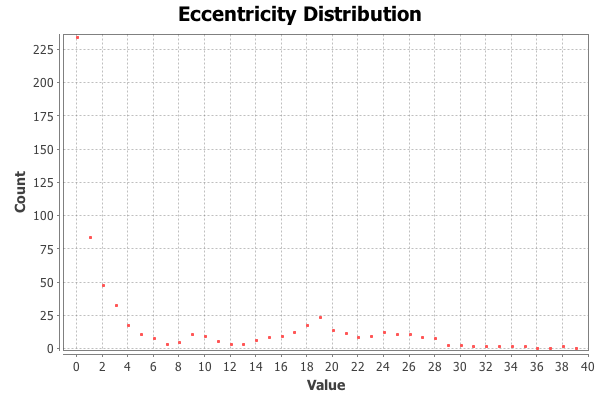
\includegraphics[scale=0.3]{plots/scribe_ecc_distr_tw}
% }
%     \subfigure[PolderCast (Facebook)]{
%     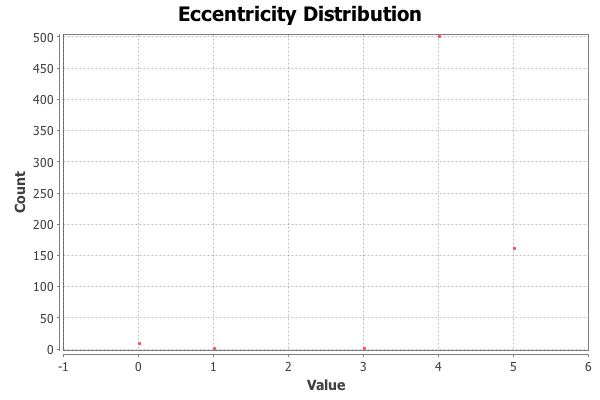
\includegraphics[scale=0.3]{plots/polder_ecc_distr_face}
% }
%     \subfigure[Scribe (Facebook)]{
%     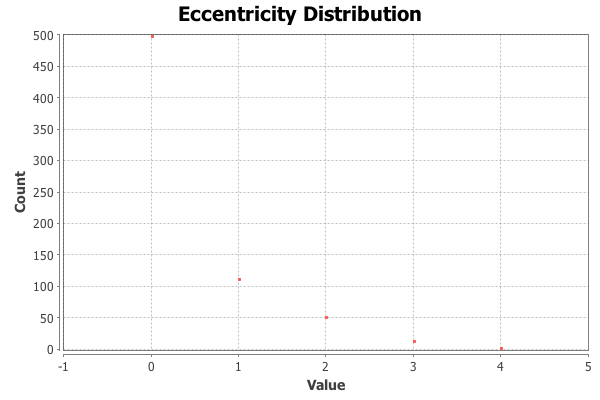
\includegraphics[scale=0.3]{plots/scribe_ecc_distr_face}
% }
%     \label{fig:betw_distr}
%     \caption{Plots showing distribution of eccentricity in PolderCast and
%     Scribe at reporter interval 1000}
% \end{figure}

\begin{figure}[H]
    \centering
    % GNUPLOT: LaTeX picture with Postscript
\begingroup
  \makeatletter
  \providecommand\color[2][]{%
    \GenericError{(gnuplot) \space\space\space\@spaces}{%
      Package color not loaded in conjunction with
      terminal option `colourtext'%
    }{See the gnuplot documentation for explanation.%
    }{Either use 'blacktext' in gnuplot or load the package
      color.sty in LaTeX.}%
    \renewcommand\color[2][]{}%
  }%
  \providecommand\includegraphics[2][]{%
    \GenericError{(gnuplot) \space\space\space\@spaces}{%
      Package graphicx or graphics not loaded%
    }{See the gnuplot documentation for explanation.%
    }{The gnuplot epslatex terminal needs graphicx.sty or graphics.sty.}%
    \renewcommand\includegraphics[2][]{}%
  }%
  \providecommand\rotatebox[2]{#2}%
  \@ifundefined{ifGPcolor}{%
    \newif\ifGPcolor
    \GPcolortrue
  }{}%
  \@ifundefined{ifGPblacktext}{%
    \newif\ifGPblacktext
    \GPblacktexttrue
  }{}%
  % define a \g@addto@macro without @ in the name:
  \let\gplgaddtomacro\g@addto@macro
  % define empty templates for all commands taking text:
  \gdef\gplbacktext{}%
  \gdef\gplfronttext{}%
  \makeatother
  \ifGPblacktext
    % no textcolor at all
    \def\colorrgb#1{}%
    \def\colorgray#1{}%
  \else
    % gray or color?
    \ifGPcolor
      \def\colorrgb#1{\color[rgb]{#1}}%
      \def\colorgray#1{\color[gray]{#1}}%
      \expandafter\def\csname LTw\endcsname{\color{white}}%
      \expandafter\def\csname LTb\endcsname{\color{black}}%
      \expandafter\def\csname LTa\endcsname{\color{black}}%
      \expandafter\def\csname LT0\endcsname{\color[rgb]{1,0,0}}%
      \expandafter\def\csname LT1\endcsname{\color[rgb]{0,1,0}}%
      \expandafter\def\csname LT2\endcsname{\color[rgb]{0,0,1}}%
      \expandafter\def\csname LT3\endcsname{\color[rgb]{1,0,1}}%
      \expandafter\def\csname LT4\endcsname{\color[rgb]{0,1,1}}%
      \expandafter\def\csname LT5\endcsname{\color[rgb]{1,1,0}}%
      \expandafter\def\csname LT6\endcsname{\color[rgb]{0,0,0}}%
      \expandafter\def\csname LT7\endcsname{\color[rgb]{1,0.3,0}}%
      \expandafter\def\csname LT8\endcsname{\color[rgb]{0.5,0.5,0.5}}%
    \else
      % gray
      \def\colorrgb#1{\color{black}}%
      \def\colorgray#1{\color[gray]{#1}}%
      \expandafter\def\csname LTw\endcsname{\color{white}}%
      \expandafter\def\csname LTb\endcsname{\color{black}}%
      \expandafter\def\csname LTa\endcsname{\color{black}}%
      \expandafter\def\csname LT0\endcsname{\color{black}}%
      \expandafter\def\csname LT1\endcsname{\color{black}}%
      \expandafter\def\csname LT2\endcsname{\color{black}}%
      \expandafter\def\csname LT3\endcsname{\color{black}}%
      \expandafter\def\csname LT4\endcsname{\color{black}}%
      \expandafter\def\csname LT5\endcsname{\color{black}}%
      \expandafter\def\csname LT6\endcsname{\color{black}}%
      \expandafter\def\csname LT7\endcsname{\color{black}}%
      \expandafter\def\csname LT8\endcsname{\color{black}}%
    \fi
  \fi
  \setlength{\unitlength}{0.0500bp}%
  \begin{picture}(7200.00,5040.00)%
    \gplgaddtomacro\gplbacktext{%
      \csname LTb\endcsname%
      \put(946,704){\makebox(0,0)[r]{\strut{} 0}}%
      \csname LTb\endcsname%
      \put(946,1111){\makebox(0,0)[r]{\strut{} 0.5}}%
      \csname LTb\endcsname%
      \put(946,1518){\makebox(0,0)[r]{\strut{} 1}}%
      \csname LTb\endcsname%
      \put(946,1925){\makebox(0,0)[r]{\strut{} 1.5}}%
      \csname LTb\endcsname%
      \put(946,2332){\makebox(0,0)[r]{\strut{} 2}}%
      \csname LTb\endcsname%
      \put(946,2740){\makebox(0,0)[r]{\strut{} 2.5}}%
      \csname LTb\endcsname%
      \put(946,3147){\makebox(0,0)[r]{\strut{} 3}}%
      \csname LTb\endcsname%
      \put(946,3554){\makebox(0,0)[r]{\strut{} 3.5}}%
      \csname LTb\endcsname%
      \put(946,3961){\makebox(0,0)[r]{\strut{} 4}}%
      \csname LTb\endcsname%
      \put(946,4368){\makebox(0,0)[r]{\strut{} 4.5}}%
      \csname LTb\endcsname%
      \put(946,4775){\makebox(0,0)[r]{\strut{} 5}}%
      \csname LTb\endcsname%
      \put(1078,484){\makebox(0,0){\strut{} 0}}%
      \csname LTb\endcsname%
      \put(1536,484){\makebox(0,0){\strut{} 100}}%
      \csname LTb\endcsname%
      \put(1994,484){\makebox(0,0){\strut{} 200}}%
      \csname LTb\endcsname%
      \put(2452,484){\makebox(0,0){\strut{} 300}}%
      \csname LTb\endcsname%
      \put(2910,484){\makebox(0,0){\strut{} 400}}%
      \csname LTb\endcsname%
      \put(3369,484){\makebox(0,0){\strut{} 500}}%
      \csname LTb\endcsname%
      \put(3827,484){\makebox(0,0){\strut{} 600}}%
      \csname LTb\endcsname%
      \put(4285,484){\makebox(0,0){\strut{} 700}}%
      \csname LTb\endcsname%
      \put(4743,484){\makebox(0,0){\strut{} 800}}%
      \csname LTb\endcsname%
      \put(5201,484){\makebox(0,0){\strut{} 900}}%
      \csname LTb\endcsname%
      \put(5659,484){\makebox(0,0){\strut{} 1000}}%
      \put(5791,704){\makebox(0,0)[l]{\strut{} 0}}%
      \put(5791,1111){\makebox(0,0)[l]{\strut{} 100}}%
      \put(5791,1518){\makebox(0,0)[l]{\strut{} 200}}%
      \put(5791,1925){\makebox(0,0)[l]{\strut{} 300}}%
      \put(5791,2332){\makebox(0,0)[l]{\strut{} 400}}%
      \put(5791,2740){\makebox(0,0)[l]{\strut{} 500}}%
      \put(5791,3147){\makebox(0,0)[l]{\strut{} 600}}%
      \put(5791,3554){\makebox(0,0)[l]{\strut{} 700}}%
      \put(5791,3961){\makebox(0,0)[l]{\strut{} 800}}%
      \put(5791,4368){\makebox(0,0)[l]{\strut{} 900}}%
      \put(5791,4775){\makebox(0,0)[l]{\strut{} 1000}}%
      \put(176,2739){\rotatebox{-270}{\makebox(0,0){\strut{}Closeness Centrality}}}%
      \put(6692,2739){\rotatebox{-270}{\makebox(0,0){\strut{}Network Size}}}%
      \put(3368,154){\makebox(0,0){\strut{}Reporter Intervals}}%
    }%
    \gplgaddtomacro\gplfronttext{%
      \csname LTb\endcsname%
      \put(4672,1757){\makebox(0,0)[r]{\strut{}PolderCast (Facebook)}}%
      \csname LTb\endcsname%
      \put(4672,1537){\makebox(0,0)[r]{\strut{}PolderCast (Twitter)}}%
      \csname LTb\endcsname%
      \put(4672,1317){\makebox(0,0)[r]{\strut{}Scribe (Facebook)}}%
      \csname LTb\endcsname%
      \put(4672,1097){\makebox(0,0)[r]{\strut{}Scribe (Twitter)}}%
      \csname LTb\endcsname%
      \put(4672,877){\makebox(0,0)[r]{\strut{}Network Size}}%
    }%
    \gplbacktext
    \put(0,0){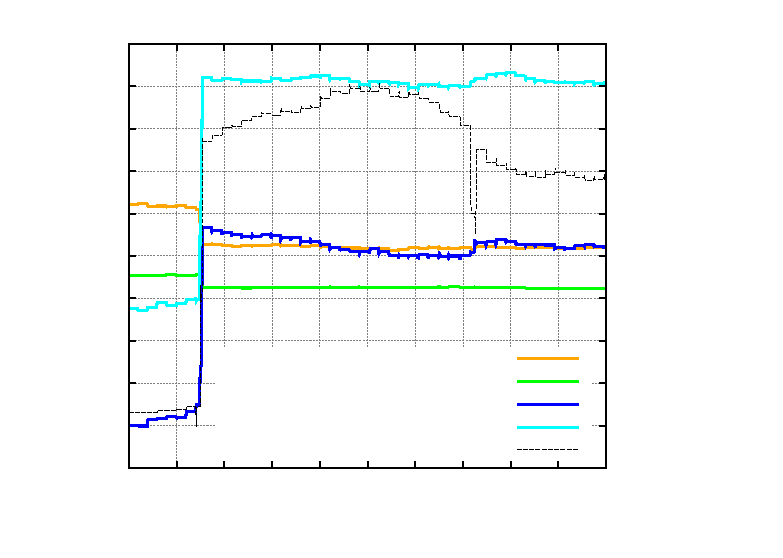
\includegraphics{eval_closeness}}%
    \gplfronttext
  \end{picture}%
\endgroup

    \caption{Avg. Closeness Centrality of PolderCast and Scribe}
    \label{fig:eval_closeness}
\end{figure}

\begin{figure}[H]
    \centering
    % GNUPLOT: LaTeX picture with Postscript
\begingroup
  \makeatletter
  \providecommand\color[2][]{%
    \GenericError{(gnuplot) \space\space\space\@spaces}{%
      Package color not loaded in conjunction with
      terminal option `colourtext'%
    }{See the gnuplot documentation for explanation.%
    }{Either use 'blacktext' in gnuplot or load the package
      color.sty in LaTeX.}%
    \renewcommand\color[2][]{}%
  }%
  \providecommand\includegraphics[2][]{%
    \GenericError{(gnuplot) \space\space\space\@spaces}{%
      Package graphicx or graphics not loaded%
    }{See the gnuplot documentation for explanation.%
    }{The gnuplot epslatex terminal needs graphicx.sty or graphics.sty.}%
    \renewcommand\includegraphics[2][]{}%
  }%
  \providecommand\rotatebox[2]{#2}%
  \@ifundefined{ifGPcolor}{%
    \newif\ifGPcolor
    \GPcolortrue
  }{}%
  \@ifundefined{ifGPblacktext}{%
    \newif\ifGPblacktext
    \GPblacktexttrue
  }{}%
  % define a \g@addto@macro without @ in the name:
  \let\gplgaddtomacro\g@addto@macro
  % define empty templates for all commands taking text:
  \gdef\gplbacktext{}%
  \gdef\gplfronttext{}%
  \makeatother
  \ifGPblacktext
    % no textcolor at all
    \def\colorrgb#1{}%
    \def\colorgray#1{}%
  \else
    % gray or color?
    \ifGPcolor
      \def\colorrgb#1{\color[rgb]{#1}}%
      \def\colorgray#1{\color[gray]{#1}}%
      \expandafter\def\csname LTw\endcsname{\color{white}}%
      \expandafter\def\csname LTb\endcsname{\color{black}}%
      \expandafter\def\csname LTa\endcsname{\color{black}}%
      \expandafter\def\csname LT0\endcsname{\color[rgb]{1,0,0}}%
      \expandafter\def\csname LT1\endcsname{\color[rgb]{0,1,0}}%
      \expandafter\def\csname LT2\endcsname{\color[rgb]{0,0,1}}%
      \expandafter\def\csname LT3\endcsname{\color[rgb]{1,0,1}}%
      \expandafter\def\csname LT4\endcsname{\color[rgb]{0,1,1}}%
      \expandafter\def\csname LT5\endcsname{\color[rgb]{1,1,0}}%
      \expandafter\def\csname LT6\endcsname{\color[rgb]{0,0,0}}%
      \expandafter\def\csname LT7\endcsname{\color[rgb]{1,0.3,0}}%
      \expandafter\def\csname LT8\endcsname{\color[rgb]{0.5,0.5,0.5}}%
    \else
      % gray
      \def\colorrgb#1{\color{black}}%
      \def\colorgray#1{\color[gray]{#1}}%
      \expandafter\def\csname LTw\endcsname{\color{white}}%
      \expandafter\def\csname LTb\endcsname{\color{black}}%
      \expandafter\def\csname LTa\endcsname{\color{black}}%
      \expandafter\def\csname LT0\endcsname{\color{black}}%
      \expandafter\def\csname LT1\endcsname{\color{black}}%
      \expandafter\def\csname LT2\endcsname{\color{black}}%
      \expandafter\def\csname LT3\endcsname{\color{black}}%
      \expandafter\def\csname LT4\endcsname{\color{black}}%
      \expandafter\def\csname LT5\endcsname{\color{black}}%
      \expandafter\def\csname LT6\endcsname{\color{black}}%
      \expandafter\def\csname LT7\endcsname{\color{black}}%
      \expandafter\def\csname LT8\endcsname{\color{black}}%
    \fi
  \fi
  \setlength{\unitlength}{0.0500bp}%
  \begin{picture}(7200.00,5040.00)%
    \gplgaddtomacro\gplbacktext{%
      \csname LTb\endcsname%
      \put(814,704){\makebox(0,0)[r]{\strut{} 0}}%
      \csname LTb\endcsname%
      \put(814,1111){\makebox(0,0)[r]{\strut{} 1}}%
      \csname LTb\endcsname%
      \put(814,1518){\makebox(0,0)[r]{\strut{} 2}}%
      \csname LTb\endcsname%
      \put(814,1925){\makebox(0,0)[r]{\strut{} 3}}%
      \csname LTb\endcsname%
      \put(814,2332){\makebox(0,0)[r]{\strut{} 4}}%
      \csname LTb\endcsname%
      \put(814,2740){\makebox(0,0)[r]{\strut{} 5}}%
      \csname LTb\endcsname%
      \put(814,3147){\makebox(0,0)[r]{\strut{} 6}}%
      \csname LTb\endcsname%
      \put(814,3554){\makebox(0,0)[r]{\strut{} 7}}%
      \csname LTb\endcsname%
      \put(814,3961){\makebox(0,0)[r]{\strut{} 8}}%
      \csname LTb\endcsname%
      \put(814,4368){\makebox(0,0)[r]{\strut{} 9}}%
      \csname LTb\endcsname%
      \put(814,4775){\makebox(0,0)[r]{\strut{} 10}}%
      \csname LTb\endcsname%
      \put(946,484){\makebox(0,0){\strut{} 0}}%
      \csname LTb\endcsname%
      \put(1417,484){\makebox(0,0){\strut{} 100}}%
      \csname LTb\endcsname%
      \put(1889,484){\makebox(0,0){\strut{} 200}}%
      \csname LTb\endcsname%
      \put(2360,484){\makebox(0,0){\strut{} 300}}%
      \csname LTb\endcsname%
      \put(2831,484){\makebox(0,0){\strut{} 400}}%
      \csname LTb\endcsname%
      \put(3303,484){\makebox(0,0){\strut{} 500}}%
      \csname LTb\endcsname%
      \put(3774,484){\makebox(0,0){\strut{} 600}}%
      \csname LTb\endcsname%
      \put(4245,484){\makebox(0,0){\strut{} 700}}%
      \csname LTb\endcsname%
      \put(4716,484){\makebox(0,0){\strut{} 800}}%
      \csname LTb\endcsname%
      \put(5188,484){\makebox(0,0){\strut{} 900}}%
      \csname LTb\endcsname%
      \put(5659,484){\makebox(0,0){\strut{} 1000}}%
      \put(5791,704){\makebox(0,0)[l]{\strut{} 0}}%
      \put(5791,1111){\makebox(0,0)[l]{\strut{} 100}}%
      \put(5791,1518){\makebox(0,0)[l]{\strut{} 200}}%
      \put(5791,1925){\makebox(0,0)[l]{\strut{} 300}}%
      \put(5791,2332){\makebox(0,0)[l]{\strut{} 400}}%
      \put(5791,2740){\makebox(0,0)[l]{\strut{} 500}}%
      \put(5791,3147){\makebox(0,0)[l]{\strut{} 600}}%
      \put(5791,3554){\makebox(0,0)[l]{\strut{} 700}}%
      \put(5791,3961){\makebox(0,0)[l]{\strut{} 800}}%
      \put(5791,4368){\makebox(0,0)[l]{\strut{} 900}}%
      \put(5791,4775){\makebox(0,0)[l]{\strut{} 1000}}%
      \put(176,2739){\rotatebox{-270}{\makebox(0,0){\strut{}Eccentricity Centrality}}}%
      \put(6692,2739){\rotatebox{-270}{\makebox(0,0){\strut{}Network Size}}}%
      \put(3302,154){\makebox(0,0){\strut{}Reporter Intervals}}%
    }%
    \gplgaddtomacro\gplfronttext{%
      \csname LTb\endcsname%
      \put(4672,1757){\makebox(0,0)[r]{\strut{}PolderCast (Facebook)}}%
      \csname LTb\endcsname%
      \put(4672,1537){\makebox(0,0)[r]{\strut{}PolderCast (Twitter)}}%
      \csname LTb\endcsname%
      \put(4672,1317){\makebox(0,0)[r]{\strut{}Scribe (Facebook)}}%
      \csname LTb\endcsname%
      \put(4672,1097){\makebox(0,0)[r]{\strut{}Scribe (Twitter)}}%
      \csname LTb\endcsname%
      \put(4672,877){\makebox(0,0)[r]{\strut{}Network Size}}%
    }%
    \gplbacktext
    \put(0,0){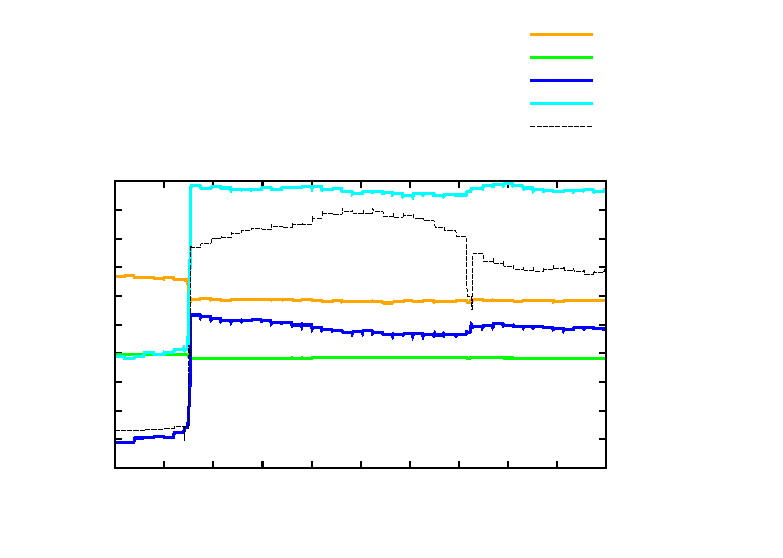
\includegraphics{eval_eccentricity}}%
    \gplfronttext
  \end{picture}%
\endgroup

    \caption{Avg. Eccentricity Centrality of PolderCast and Scribe}
    \label{fig:eval_eccentricity}
\end{figure}

